%\documentclass{article}
\title{ECE 397 Research Report}
\author{
        Bhargava Manja \\
        manja2@illinois.edu\\
}
\date{\today}

\documentclass[11pt]{article}
\usepackage[pdftex]{graphicx}
\usepackage{listings}
\usepackage{float}
\usepackage{titling}
\usepackage{subfigure}
\usepackage{url}

\begin{document}
\maketitle

\section{Introduction}
This report aims to summarize my work with the DEPEND research group from
October 2014 to December 2014. I first discuss the background of the project,
and in Section II I present an overview of concolic execution, followed by a
brief review of related literature in Section III. This is followed by overviews
of technologies used in this project, and finally by an description of the
conclusions gathered this semester and plans for future work. 

\subsection{Background}
My research aims to use concolic execution to
test the KVM hypervisor. In the context of this work, \textit{concolic
execution} is a testing technique that performs symbolic execution, which
treats program variables as symbolic values, along concrete execution
paths. By combining symbolic execution, which can test whole classes of
inputs at once, with selective concrete execution, we can test a large number of
machine states and catch bugs that are simply impractical to find with unit
tests \par
 
I met with Zak and Cuong late last semester about working with DEPEND, but the
process of selecting a project did not begin until early this semester. After
much discussion, we chose to work on using concolic execution to test parts of
KVM, due to my interest in programming languages and symbolic execution. \par
This
semester, I focused on understanding S2E, the concolic execution engine we
decided to use, and how it could be used to test KVM. Due to time constraints
and the process of learning, I performed mostly exploratory work, which will be
expanded upon next semester.

\subsection{Timeline}
Details on each of the following items are presented throughout the rest of the
report
\begin{itemize}
\item Joined the group and discussed potential projects
\item Began learning about concolic execution, the architecture of KVM, and S2E,
  a concolic execution engine that was to be used for the project
\item Set up a Linux machine and completed a majority of the S2E tutorials
\item Studied the implementation of AMD SVM support in QEMU to ascertain whether
  it would be feasible to add support for the Intel VT-X instruction set
\item Created a two tiered testing setup to test KVM's hardware acceleration
  features with S2E
\item Identified code paths to begin instrumentation for S2E's concolic
  execution engine
\end{itemize}

\section{Concolic Execution}
In \textit{unit testing}, programs are decomposed into functional units which
are individually tested by generating inputs to functions that serve as entry
points. Thus, assuming a collection of unit tests cover all code paths, the
quality of testing reduces to the quality of test inputs. Manual generation of
values leads to incomplete testing and necessitates changing inputs whenever the
system changes, which is impractical. \par
Several techniques are used to automate
the production of high quality testing inputs. One scheme randomly chooses
values from the space of possible inputs. This has two serious problems: first,
many values may lead to the same states and behaviour, and second, the
probability of selecting inputs that lead to bad states and buggy behaviour is
often incredibly small, especially for any sizeable real world system that may
have millions of discrete states. \par
Another approach that eliminates redundant
test input and improves code coverage is \textit{symbolic execution}, in which a
program is executed with symbolic values as input. Each conditional expression
represents a constraint that determines an execution path. Thus, the states of
the program can be represented as an execution tree, where internal nodes
represent conditional branches. By generating concrete values, we want to
explore all the paths in the tree. However, as you can imagine, for any large
software system the size of the execution tree is intractably large, and so can
not be explored purely symbolically. A program with just ten binary branches
yields $2^{10}$ different states. \par
First proposed by Larson and Astin, \textit{concolic execution} modifies the concept of symbolic execution to
exploit its advantages while avoiding the combinatorial explosion of program
states. With this approach, concrete execution accrues constraints at every
branch point. These constraints are solved to generate new concrete inputs that
direct execution along new paths. This idea has been refined, notably by
Godefroid et. al and Sen, Marinov, and Agha here at the University of Illinois. 

\section{Literature Review}
Work has been done by other researchers pertaining to the use of concolic
execution in testing. In particular, previous related work
tends to focus on one of the following:
\begin{itemize}
\item Strategies to increase the effectiveness of concolic execution as a bug
finding tool
\item Concolic execution based testing of different classes of applications
\end{itemize}

\subsection{Increasing Testing Effectiveness}
Because of both the inherent inefficiency of using and keeping track of symbolic
variables during program execution, much work has been done for the purpose of
making concolic testing more efficient. Inefficiencies exist because of the
sheer size of the space of possible program states. Many methods have been
developed to prune the state tree. Flanagan and Godefroid introduce the idea
of \textit{partial order reduction}, which identifies branches that do not
depend on each other and utilizes concurrency to speed exploration and execution
of these branches. The ``Boosting Concolic Testing'' paper develops the idea
of \textit{interpolation}, which uses code annotations to ignore code paths that
are guaranteed to not hit any bugs, thus greatly reducing the state tree. Seo
and Kim created the idea of \textit{context guided search}, a method for
choosing branches to explore based on the how the current branch was
reached. Experiments presented in all these papers show orders of magnitude
decreases in the amount of branches searched to reach a target code coverage. 

\subsection{Testing Different Applications}
Much of the work around concolic testing has involved applying the technique to
different problem domains. For example, the Jalangi paper implements concolic testing for
Javascript applications in the browser. The Sarkar paper discusses the use of
concolic testing to test both the host language and query language of a SQL
database application. All this work highlights the extensability of the methods
used in this project, and offers clues on how to improve the testing of KVM.

\section{QEMU}
QEMU, short for ``quick emulator'', is a program that enables pure software
machine emulation via fast binary translation. When combined with KVM, it can
harness processor support for virtualization and provide hardware
acceleration. It underlies both S2E and the setup for this project.
\subsection{Exploring Modifications to QEMU}
A significant amount of time this semester was spent examining whether we could
add support in QEMU for Intel's VT-x instructions. QEMU supports AMD's SVM
instructions, so I studied this implementation to determine how feasible
extending it to VT-x would be. The implementation was mostly confined to 4
files:
\begin{enumerate}
\item target-i386/svm.h: Contains data structures that implement the Virtual
Machine Code Block, which contains VM state and initialization information, as
well as space for state to be saved on VMEXITs
\item target-i386/svm\textunderscore helper.c: All the SVM instructions are implemented here as
functions with signature helper\textunderscore <instruction>
\item target-i386/helper.c: Uses QEMU macros to register functions in
svn\textunderscore helper.c with one of QEMU's many dispatchers
\item target-i386/translate.c: Massive switch case block that acts like a state
machine, calls relevant SVM functions. Calls to those functions go through
gen\textunderscore helper \textunderscore <instruction> functions that appear
nowhere else. These stubs are points where the Tiny Code Generator is used to
generate actual machine code. 
\end{enumerate}
Due to the complexity of the SVM implementation (which
involves runtime function registration and code generation), and the fact that
utilizing the SVM implementation was as simple as changing the OS and emulated
CPU type in experiments, we decided against modifying QEMU.

\section{S2E}
S2E is a platform for analyzing the behaviour of large and complex software
systems with concolic execution. S2E uses virtualization to allow
analysis during normal operation of the tested software, unlike other tools
which use models or stubs. S2E also performs binary translation, allowing it to
execute directly on binaries. Two important concepts of S2E
are \textit{selectors} and \textit{analyzers}. S2E performs automated path exploration by executing
code paths in parallel, but for the sake of efficiency it tries to only execute
paths that are of interest with regards to the intent of the testing being
performed. Selectors guide exploration by specifying paths of interest. For
example, we may be interested in all paths that touch a specific memory object,
paths influenced by a specific parameter, paths inside a target code module,
etc. During exploration, analyzers collect information or check that the desired
properties of a path (to look for bugs). S2E comes with many stock selectors and
analyzers, but they can also be written from scratch with the S2E API. \par
The typical S2E user only needs to define in a configuration file the desired
selectors and analyzers along with the corresponding parameters, start up the
desired software stack inside the S2E virtual machine, and run the S2E launcher
in the guest OS, which starts the desired application and communicates with the
S2E VM underneath via custom S2E opcodes. \par
The S2E paper provides the example of trying to verify the code that handles
license keys in a proprietary program, such as Adobe Photoshop. The user
installs the program in the S2E Windows VM and launches the program using
s2e.exe. From inside the guest OS, the s2e.exe
launcher communicates with S2E. In the S
2E configuration file, the tester may choose a memory-checker analyzer along
with a path selector that returns a symbolic string whenever Photoshop reads
a specific registry entry from the Windows registry. S2E
then automatically explores the code paths in Photoshop that are influenced by
the value of the license key and looks for memory safety errors along those 
paths. \par
\subsection{S2E Opcodes}
S2E opcodes are custom binary opcodes inserted into S2E VM guest programs, and
which are directly interpreted by S2E. They do things like making values
symbolic, logging debug information, enabling multipath execution, etc. The
simplest way of inserting them into a program is to use the higher level S2E C
API, defined in the file s2e.h, which comes with the S2E distribution. This
requires sight modification to the target program.
A simple example of a modified program is shown below:
\begin{figure}[htp]
\begin{verbatim}
#include <stdio.h>
#include <string.h>
#include "s2e.h"

int main(void)
{
  char str[3];

  s2e_enable_forking();
  s2e_make_symbolic(str, 2, "str");

  if(str[0] == '\n' || str[1] == '\n') {
    printf("Not enough characters\n");
  } else {
    if(str[0] >= 'a' && str[0] <= 'z')
      printf("First char is lowercase\n");
    else
      printf("First char is not lowercase\n");

    if(str[0] >= '0' && str[0] <= '9')
      printf("First char is a digit\n");
    else
      printf("First char is not a digit\n");

    if(str[0] == str[1])
      printf("First and second chars are the same\n");
    else
      printf("First and second chars are not the same\n");
  }

  s2e_disable_forking();

  s2e_get_example(str, 2);
  printf("'%c%c' %02x %02x\n", str[0], str[1],
         (unsigned char) str[0], (unsigned char) str[1]);

  return 0;
}
\end{verbatim}
\caption{An example of a small program modified with S2E instructions}
\end{figure}
\newpage
This simple program has been modified to make the str variable symbolic. By
enabling forking, we tell S2E to explore the different states that can be
reached in each of the branches introduced by the conditional
statements. Finally, the call to s2e\textunderscore get\textunderscore example
solves the accrued path constraints to generate a concrete value indicative of a
possible end value of the str variable. A more direct route, when the source
code of a target program is not available, is to directly modify a compiled
binary with S2E opcodes.

\subsection{Selective Symbolic Execution}
The killer feature of S2E (and any concolic analysis tool) is its ability to
drastically reduce the analyzed state space of a program with \textit{selective
symbolic execution}. The idea is to treat a program as a superposition of all
possible execution paths, which we can visualize as a tree, with each root -
leaf path corresponding to an execution path. Then, variables can thought of as
superpositions of all possible values they can take instead of concrete
values. Any time a branch depends on some symbolic variable $x$, we split
execution into two different executions, each with $x$ constrained s required to
cause the branch to take that path. This process continues recursively, with
paths executed in parallel. Only some of these paths actually matter; many can
be ignored without effecting the quality of testing or analysis. Thus, S2E
performs \textit{transitions} between symbolic and concrete execution. The
symbolic execution is reserved for paths and sections that we care about. For
example, if we wish to test a shared library, but don't care about execution
paths through applications that use that library or the kernel, our execution
tree might look something like this:
\begin{figure}[htp]
\centering
        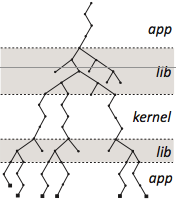
\includegraphics{exec_tree}
\caption{An example of an execution tree. Symbolic execution occurs in the
shaded areas}
\end{figure}
\newpage
There are two kinds of transitions: from concrete to symbolic and from symbolic
to concrete. In the above example, this type of transition would occur when app
calls into lib with a concrete argument. This argument is made symbolic,
possibly with constrains (for example, $x > 20, x \% 2 == 0$). Lib is executed
both symbolically and concretely, with the concrete argument from app. When lib
is finished, the concrete value from the concrete execution is returned to app,
but lib has been explored symbolically as well. \par
The transition from symbolic to concrete is slightly more complicated. Simply
put, when a symbolic variable needs to be made concrete (for output or writing
to disk, for example), its \textit{path constraints} (constraints on the
variable that are required for this particular execution point to be reached)
are solved, yielding a concrete value. This value is added to the path
constraints, for the sake of correctness (because the further execution of the
path depends on the concrete value in some way). 

\subsection{Architecture of S2E}
S2E depends on parts of QEMU, the KLEE symbolic execution engine, and LLVM. S2E
explores paths by executing a target program in a virtual machine and executing
paths of interest symbolically, as discussed previously. QEMU is used to perform
dynamic binary translation of the target program and system. During concrete
execution, the end product of the dynamic translation is executed by the host
machine's physical CPU. During symbolic execution, guest instructions (including
S2E opcodes) are translated into LLVM IR and executed by KLEE. S2E transparently
converts data between symbolic and concrete formats, providing the illusion of
full symbolic execution. The following diagram shows the different parts of the
S2E system:
\begin{figure}[htp]
\centering
    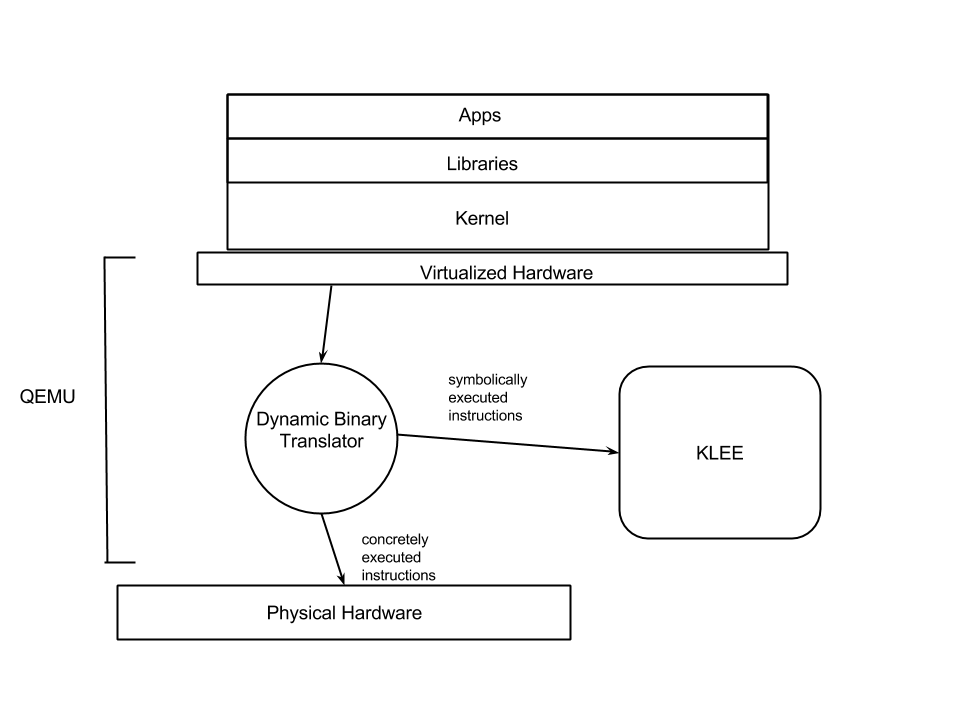
\includegraphics[scale=.3]{s2e_arch}
\caption{An illustration of the S2E system}
\end{figure}
\newpage
The nature of S2E creates a unique challenge with regards to this project. We
want to test parts of KVM, which executes some guest instructions on physical
CPUs with virtualization instructions (VT-x or SVM). This is not suitable for
direct analysis with S2E, as S2E needs to translate all instructions into LLVM IR
for analysis with KLEE, and the translation of virtualization instructions is
not supported. Thus, in the next few 
sections, I explain the testing environment developed for this project. 

\subsection{Using S2E}
The goal for this project is to use S2E to examine all possible VMEXIT states to
look for bugs. Given the complexity of the systems at play, it is impossible to
do any sort of reasonable analysis using unit testing (too little code coverage)
or symbolic execution (too many possible states). By leveraging the power of
concolic execution, we can enjoy the benefits of symbolic execution while
getting around the issue of combinatorial explosion in the state space. \par

The challenge now is to design experiments that get around the problem of state
space explosion while providing meaningful results and insight. One method we
have tried is to make symbolic values that, while important to the function of
KVM, are not so widely used that they force the analysis of a huge number of
states. For example, the very first experiment used the 'exit\textunderscore
code' field of the VMCB. This field is used by KVM to determine what caused a
VMEXIT, and to handle errors. Thus it is important in directing the program flow
of KVM and QEMU, but it is only read and written to in a small number of
locations. Thus, the modifications required are extremely simple. Below is a
graphical depiction of what we aim to do:
\begin{figure}[htp]
\centering
    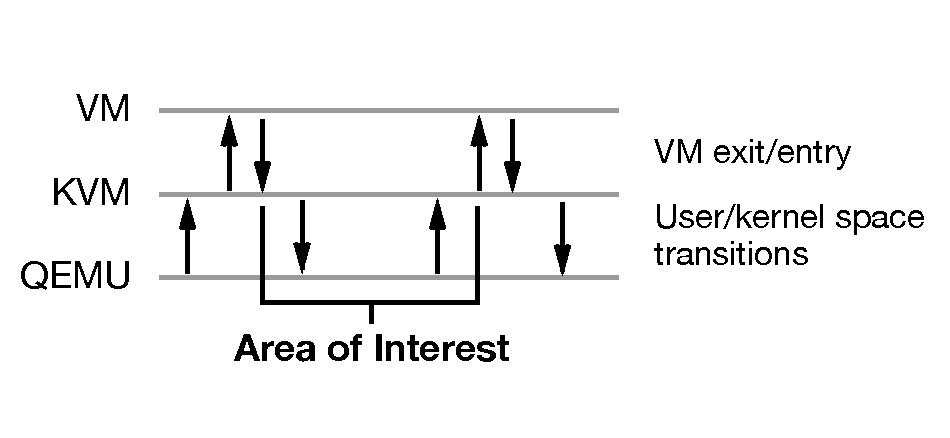
\includegraphics[scale=.7]{qemu_trap.pdf}
\end{figure}
\newpage
By instrumenting the code that determines behavior in the highlighted area of
operation, we hope to find bugs that are impractical to find without the aid of
concolic execution.


\section{Testing Setup}
I set up the testbed for running S2E experiments on Strauss. After creating a
raw 5GB disk image, I installed Ubuntu 12.04, then used LVM (Logical Volume
Manager) to increase the disk space and copied the original disk image into the
VM. I run the outer VM with KVM disabled and SVM enabled, log in, and launch the
inner VM with KVM enabled. This allows us to test KVM with S2E. A figure
illustrating the testing environment follows:
\begin{figure}[htp]
\centering
    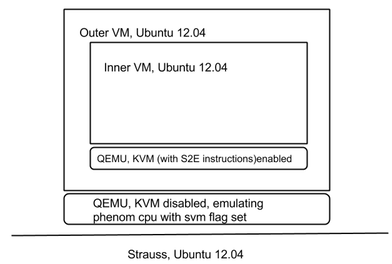
\includegraphics[scale=.7]{test_setup}
\caption{The environment developed for running experiments}
\end{figure}
\newpage
This setup gets around the problem of S2E's lack of support for symbolic
execution of virtualization instructions. KVM is disabled in the first layer so
that symbolic execution will work, and is enabled in the second layer so that
KVM can be symbolically executed. Now, KVM instructions are emulated by QEMU,
and so can be symbolically executed. 
\par

To actually run experiments, I had to identify two things:
\begin{enumerate}
\item The location of VMEXIT handlers in KVM
\item The 'parameters' that determined behavior at those locations
\end{enumerate}

The first location I found was in the KVM svm implementation. The only parameter
of this location is the VM Control Block, which consists of many fields. Thus,
the first experiment performed will be to analyze the behavior of KVM when the
VMCB exit code field is made symbolic - that is, we aim to examine all the
different possible code paths reached with different values of the exit code
field in the VMCB. 

\section{Conclusions}
This semester, I learned about Linux virtualization technologies and symbolic
execution as a software testing tool. Though I have some background in security,
systems, and programming language/compiler technologies, I have never worked in
the intersection of these three fields, a process which I found very
edifying. Most of my time this semester was spent learning the
technologies used in this project, exploring various avenues of inquiry, and
setting up testing environments, so I plan on using the spring semester to
gather data and quantitatively examine KVM with S2E.

\bibliographystyle{abbrv} \bibliography{main}

\end{document}
